%!TEX root = thesis.tex

\chapter{Monitorability}
\label{chapter-monitorability}
	Because of time and memory restrictions, online monitoring on a possible infinite run of a system is only reasonable, if several constraints are fulfilled. Therefore, the term of \emph{Finite Monitorability} will be introduced, which ensures, that a property can be supervised using an online monitor.

\section{Finite Monitorability}
	\subsection{Timestamps}
		\label{monitorability_timestamps}
		As we consider streams that can be infinite, the time value of events can also grow into infinity. This is problematic, because it leads to infinite memory and runtime requirements, which cannot be meet, especially not in the context of online monitoring. Therefore, the time domain $\mathbb{T}$ must be restricted by the following constraints:
		\begin{itemize}
			\item
				$\mathbb{T}$ must be discrete.
			\item
				The first used timestamp has the value $t_0=0$
			\item
				All used timestamps must be smaller than $t_{max}$.\\
				$t_{max}$ must be big enough, so it is not reached in practical use \footnote{for example, a 64-bit unsigned integer variable is enough, to cover nanoseconds for 584.55 years}.
			\item
				The distance between two subsequent time values is small enough to observe the wanted constraints.
		\end{itemize}
		%Additionally, a table $\tau \in \mathbb{T}'\times\mathbb{T}$ is defined, where $\mathbb{T}'$ is a set of indices. $\tau$ stores exactly the %timestamps, which are part of the current state of the monitor, which will be introduced in \ref{monitorability_state}. 
	\begin{figure}
		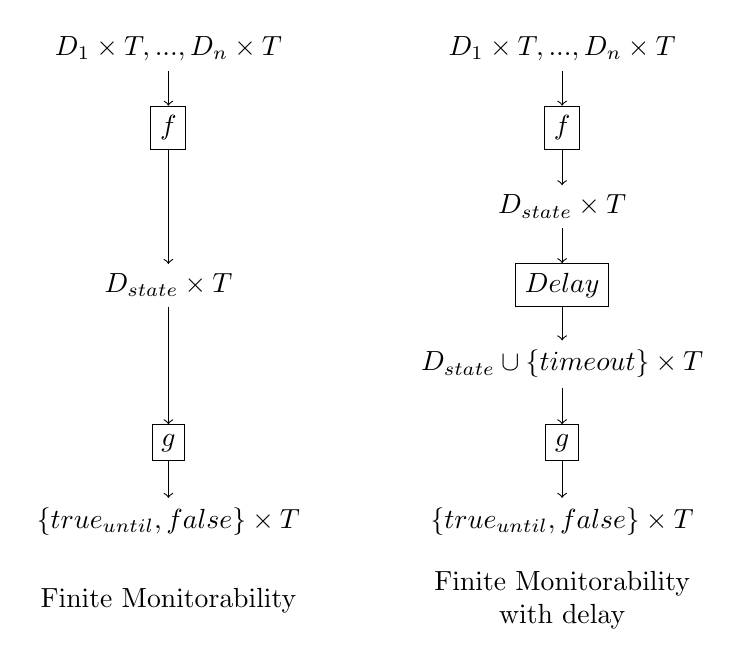
\begin{tikzpicture}
			\node[] (inputRight){$\mathbb{D}_1\times\mathbb{T}, ..., \mathbb{D}_n\times\mathbb{T}$};
			\node[draw, below of=inputRight] (fRight){$f$};
			\node[below of=fRight] (stateRight){$\mathbb{D}_{state}\times\mathbb{T}$};
			\node[draw, below of=stateRight] (delayRight){$Delay$};
			\node[below of=delayRight] (stateDelayRight){$\mathbb{D}_{state}\cup\{timeout\}\times\mathbb{T}$};
			\node[draw, below of=stateDelayRight] (gRight){$g$};
			\node[below of=gRight] (outputRight){$\{true_{until}, false\}\times\mathbb{T}$};
			\draw[->] (inputRight) -- (fRight);
			\draw[->] (fRight) -- (stateRight);
			\draw[->] (stateRight) -- (delayRight);
			\draw[->] (delayRight) -- (stateDelayRight);
			\draw[->] (stateDelayRight) -- (gRight);
			\draw[->] (gRight) -- (outputRight);
			\node [below of=outputRight, align=center] (h0){Finite Monitorability\\with delay};

			
			\node[left of = inputRight] (h1){};
			\node[left of = h1] (h2){};
			\node[left of = h2] (h3){};
			\node[left of = h3] (h4){};
			
			\node[left of = h4] (inputLeft){$\mathbb{D}_1\times\mathbb{T}, ..., \mathbb{D}_n\times\mathbb{T}$};
			\node[draw, below of=inputLeft] (fLeft){$f$};
			\node[below of = fLeft] (h5){};
			\node[below of=h5] (stateLeft){$\mathbb{D}_{state}\times\mathbb{T}$};
			\node[, below of=stateLeft] (delayLeft){};
			\node[draw, below of=delayLeft] (gLeft){$g$};
			\node[below of=gLeft] (outputLeft){$\{true_{until}, false\}\times\mathbb{T}$};
			\draw[->] (inputLeft) -- (fLeft);
			\draw[->] (fLeft) -- (stateLeft);
			\draw[->] (stateLeft) -- (gLeft);
			\draw[->] (gLeft) -- (outputLeft);
			\node [below of=outputLeft] {Finite Monitorability};
		\end{tikzpicture}
		\centering
		\caption{Overview Finite Monitorability - with or without \emph{delay}}
		\label{fig:OverviewMonitorability}
	\end{figure}
	\subsection{Finite Monitorability}
		%TODO mention figure
		For the definitions of streams and functions defined on them, TeSSLa-like syntax is used. Also, some standard TeSSLa functions are used in the definitions. 
		\subsubsection{Input Streams}
			Let $S_1, S_2, ..., S_n$ be input streams with\\
			$\forall i:$ $S_i=(\mathbb{T}\cdot \mathbb{D}_i)^\omega\cup(\mathbb{T}\cdot \mathbb{D}_i)^+\cup(\mathbb{T}\cdot \mathbb{D}_i)^*\cdot(\mathbb{T}_\infty\cup\mathbb{T}\cdot\{\bot\})$ and\\
			All types $D_i$ have a finite size.
		\subsubsection{State Stream}
			\label{monitorability_state}
			Let $S_{state}$ with\\
			$S_{state}= (\mathbb{T}\cdot \mathbb{D}_{state})^+\cup(\mathbb{T}\cdot \mathbb{D}_{state})^*$\\
			be a state stream, where $\mathbb{D}_{state}$ has a finite size.\\
			Further let $f: S_1 \times S_2 \times ... \times S_n \times S_{state}\rightarrow S_{state}\times \mathbb{T}$ a state transition function, which defines the state stream in an incremental fashion:\\
			$\forall t\in \mathbb T \exists i\in \{1,2,...,n\}: S_i(t)\in\mathbb D_i$\\
			$\rightarrow S_{state}(t)= f(S_1(t), S_2(t), ..., S_n(t), last(S_{state}, merge(S_1, S_2, ..., S_n))(t))$\\
			The runtime of $f$ is in $\mathcal{O}(1)$.
		\subsubsection{Output Stream}
			Let $S_{output}= (\mathbb{T}\cdot \{true_{until}, false\})^+\cup(\mathbb{T}\cdot \{true_{until}, false\})^*$\\
			be the output stream, which is defined via a function\\
			$g: \mathbb{D}_{state}\times \mathbb{T}\rightarrow \{true_{until}, false\}\times \mathbb{T}$\\
			The runtime of $g$ is in $\mathcal{O}(1)$.
		\subsubsection{Evaluation}
			A property of a set of streams is called \emph{Finite Monitorable}, if a function $f$ with type $\mathbb{D}_{state}$ and a function $g$ exist, which fulfill the characteristics called above, and which outputs $true_{until}$, as long as the property is fulfilled and $false$, in any other case. It should be noted that these definitions are \emph{timestamp conservative}, because the streams $S_{state}$ and $S_{output}$ can only change their data value at the timestamps of input events.
		% TODO transducer
		\subsubsection{Equivalences}
			
	\subsection{Finite Monitorability with Delay}
		%TODO mention figure
		Not all of the TADL2 constraints can be monitored in a \emph{timestamp conservative}. For example, the \emph{RepeatConstraint} with the attributes $lower=upper=4$ and $span=1$ expects subsequent events to have a time distance of $4$. If one event is missing, the output of a timestamp conservative monitor would still be $true_{until}$, until the next input event arrives. Therefore, the monitor cannot not check the constraint correctly. Because of this problem, the definition of \emph{Finite Monitorability} is expanded by the ability of introducing new timestamps.
		\subsubsection{Input Streams}
			The definition of the input streams are unchanged.
		\subsubsection{State Stream}
			The function $f$ remains unchanged, but the state stream $S_{state}$ is expanded by an \emph{timeout} value, which is inserted after a specific period of time, in which no input event has arrived.
		\subsubsection{Delay}
			A \emph{delay generator}, which copies the states produced by the function $f$ and inserts a \emph{timeout} state into the state stream, if there was no input event for a specific period of time, is added to the definition. The length of this period depends on the current state of the monitor.
		\subsubsection{Output Stream}
			The output function $g$ is expanded by the \emph{timeout} value:\\
			$g: (\mathbb{D}_{state}\cup\{timeout\})\times \mathbb{T}\rightarrow \{true_{until}, false\}\times \mathbb{T}$\\
			The definition of the output stream $S_{output}$ remains unchanged.
		\subsubsection{Evaluation}
			A property of a set of streams is called \emph{Finite Monitorable with Delay}, if a function $f$ with type $\mathbb{D}_{state}$, a delay generator and a function $g$ exist, which fulfill the characteristics called above, and which outputs $true_{until}$, as long as the property is fulfilled and $false$, in any other case.
			
	\subsection{Non-Finite Monitorability}
		Not all TADL2 constraints are finite monitorable, because a monitor would require infinite memory and/or time resources. In a theoretical view, this makes online monitoring on infinite traces impossible, because a machine with infinite resources does not exist in the real world. In a practical view, many of these problems are solved by using a system with finite memory, with the hope that this finite resources would be enough, to cover the inputs of the ''real world''. In these cases, a distinction is useful, as some constraints have resource requirements, that grow continuously with every input event, and others constraints only require infinite resources in worst case scenarios. Obviously, the constraints with continuous resource requirement growth cannot be monitored infinitely, but the constraints, that only need infinite resources, can be monitored in many cases.\\
		\\
		In the next chapter, each of the TADL2 constraints will classified into \emph{Finite Monitorable}, \emph{Finite Monitorable with Delay} and \emph{Non-Finite Monitorability}. For the last class, it will be demonstrated, if the constraint is non-finite monitorable in any cases or just in worst case scenarios.
		
		
			
		
		
	 